\item \defpoints{10} [Linear Regression and Classification]

(a) When we talk about linear regression, what does `linear' regard to? \defpoints{2}

(b) Assume that there are $n$ given training examples $\{(x_1, y_1), (x_2, y_2), \cdots, (x_n, y_n)\}$, where each input data point $x_i$ has $m$ real valued features. When $m > n$, the linear regression model is equivalent to solving an under-determined system of linear equations $\mathbf{y} = \mathbf{X}\beta$. One popular way to estimate $\beta$ is to consider the so-called ridge regression:
$$\argmin_{\beta} ||\mathbf{y}-\mathbf{X}\mathbf{\beta}||_2^2 + \lambda||\beta||_2^2$$
for some $\lambda > 0$. This is also known as Tikhonov regularization. Show that the optimal solution $\beta^*$ to the above optimization problem is given by
$$\mathbf{\beta}^* = (\mathbf{X}^{\top}\mathbf{X} + \lambda \mathbf{I})^{-1}\mathbf{X}^{\top}\mathbf{y}$$
Hint: You need to prove that given $\lambda>0$, $\mathbf{X}^{\top}\mathbf{X} + \lambda \mathbf{I}$ is invertible. \defpoints{5}

(c) Is the given data set linear separable? If yes, construct a linear hypothesis function to separate the given data set. If no, explain the reason. \defpoints{3}
\begin{table}[h]
    \centering
    \begin{tabular}{c|cccccc}
        Data & (1,3) & (4,4) & (3,-6) & (-2,1) & (-3,5) & (-6,-4) \\ \hline
        Label & +1 & -1 & -1 & +1 & -1 & -1
    \end{tabular}
    \label{tab:my_label}
\end{table}

\solution

(a) Linear is to the for all parameters of the regression variable $\beta$.

(b) As we have learned in linear algebra, we know that tha matrix $X^{\top}X$ is symmetric, which must be diagonalizable. i.e. there must exist a matrix $P$ and a diagonal matrix $\Lambda$ such that $X^{\top}X=P\Lambda P^{-1}$.\\
Also $\forall x\in\mathbb{R}^n$, we have
$$x^{\top}(\mathbf{X}^{\top}\mathbf{X}) x=(\mathbf{X}x)^{\top}(\mathbf{X}x)=\|\mathbf{X}x\|_2^2\geq0$$
So $X^{\top}X$ is positive semi-definite, which means all eigenvalues of $X^{\top}X$ are non-negative, i.e. the diagonal matrix $\Lambda$'s elements are all positive. \\
And since $\lambda>0$, so $\lambda I$'s all elements are all also non-negative, and $\lambda I$ is also a diagonal matrix. Since
$$X^{\top}X+\lambda I=P\Lambda P^{-1}+\lambda PIP^{-1}=P(\Lambda+\lambda I)P^{-1}$$
And $\Lambda, \lambda I$ are all diagonal matrix, so $\Lambda+\lambda I$ is also a diagonal matrix. And all elements in $\Lambda+\lambda I$ are all positive, so $\Lambda+\lambda I$ is positive defined. Since $X^{\top}X+\lambda I=P(\Lambda+\lambda I)P^{-1}$,
from the knowledge of similarity and diagonalizable, we could know that $X^{\top}X+\lambda I$ is also positive defined. So $X^{\top}X+\lambda I$ is invertible.

And let
$$f(\beta)=\|\mathbf{y}-\mathbf{X}\mathbf{\beta}\|_2^2 + \lambda\|\beta\|_2^2=(\mathbf{y}-\mathbf{X}\mathbf{\beta})^{\top}(\mathbf{y}-\mathbf{X}\mathbf{\beta})+\lambda\beta^{\top}\beta=\mathbf{y}^{\top}\mathbf{y}-\beta^{\top}\mathbf{X}^{\top}\mathbf{y}-\mathbf{y}^{\top}\mathbf{X}\beta+\beta^{\top}\mathbf{X}^{\top}\mathbf{X}\beta+\lambda\beta^{\top}\beta$$
Since $f(\beta)$ is convex(prove below), so we just need to set the derivative of $f(\beta)$ to 0 to get the optimal solution.
\begin{align*}
\dfrac{\partial f(\beta)}{\partial \beta} &= 2(-\mathbf{X}^{\top}\mathbf{y}+\mathbf{X}^{\top}\mathbf{X}\beta+\lambda\beta) \\
\dfrac{\partial f(\beta)}{\partial \beta}=0 &\Rightarrow (\mathbf{X}^\mathbf{X}+\lambda I)\beta=\mathbf{X}^{\top}\mathbf{y}\Rightarrow \beta=(\mathbf{X}^{\top}\mathbf{X}+\lambda I)^{-1}\mathbf{X}^{\top}\mathbf{y} \\
\nabla_{\beta}^2 f(\beta) &= 2(2\mathbf{X}^{\top}\mathbf{X}+\lambda I) \succ 0
\end{align*}
Since we have proved that $X^{\top}X+\lambda I$ is invertible, so $(\mathbf{X}^{\top}\mathbf{X}+\lambda I)^{-1}$ exists, so
$$\beta^*=(\mathbf{X}^{\top}\mathbf{X}+\lambda I)^{-1}\mathbf{X}^{\top}\mathbf{y}$$

\newpage
(c) Actually this question is not very reasonable, sorry for causing you confusions. It is better to ask are the data linear separable in the origin feature space. Then the answer is no. \\
Solution1: only consider in the origin feature space, the data is not linear separable. \\
To prove this, you may plot a figure as follows. And briefly, intuitively say that it is not seperable.
\begin{figure}[h]
    \centering
    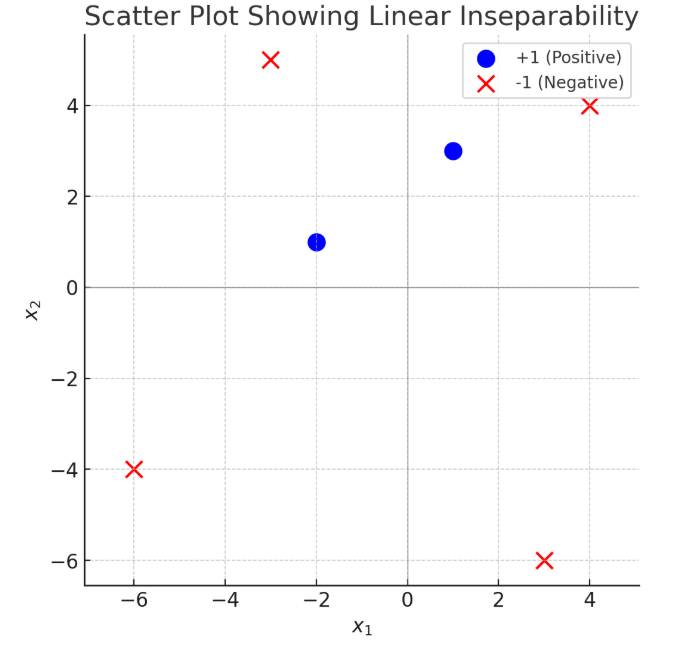
\includegraphics[width=7cm]{figure/p3.png}
\end{figure}

Or a more theoretical way:
\begin{figure}[h]
    \centering
    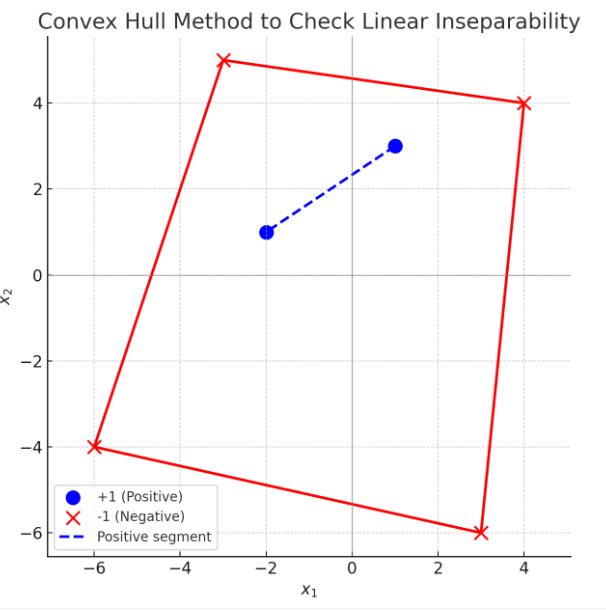
\includegraphics[width=7cm]{figure/convex_hull.png}
\end{figure}

According to the Convex Set Separation Theorem, if two sets of data points are linearly separable, the convex hulls formed by each set must not intersect, and there must exist at least one hyperplane strictly separating these convex hulls.

Conversely, if the convex hulls of the two sets of data points intersect, it implies that there is no linear hyperplane capable of strictly separating these two sets, indicating that the data is linearly inseparable in the given space.


Solution2: if we consider another feature space: \\
Let the data be formed as $\mathbf{X}_i=(x_1,x_2)$, and let the hypothesis function be $f(\mathbf{X})=b_1x_1^2+b_2x_2^2+b_3$. Let $b_1=1,b_2=1,b_3=-25$, so the regression function is $f(\mathbf{X})=x_1^2+x_2^2-25$, and its a linear regression. Make the separate line be $f(\mathbf{X})=0$, so the separate line is $x_1^2+x_2^2-25=0$. If $f(\mathbf{X})\leq 0$, set the label to be $+1$, else set the label to be $-1$. And we could get the result as below:

\begin{table}[H]
\centering
\begin{tabular}{c|cccccc}
Data $\mathbf{X}$ & (1,3) & (4,4) & (3,-6) & (-2,1) & (-3,5) & (-6,-4) \\ \hline
Function value $f(\mathbf{X})$ & -15 & 7 & 20 & -20 & 9 & 27\\
Label & +1 & -1 & -1 & +1 & -1 & -1
\end{tabular}
\label{tab:my_label}
\end{table}

So above all, we could find that we can construct a linear hypothesis function to separate the given data set.

\newpage